\documentclass[1p]{elsarticle_modified}
%\bibliographystyle{elsarticle-num}

%\usepackage[colorlinks]{hyperref}
%\usepackage{abbrmath_seonhwa} %\Abb, \Ascr, \Acal ,\Abf, \Afrak
\usepackage{amsfonts}
\usepackage{amssymb}
\usepackage{amsmath}
\usepackage{amsthm}
\usepackage{scalefnt}
\usepackage{amsbsy}
\usepackage{kotex}
\usepackage{caption}
\usepackage{subfig}
\usepackage{color}
\usepackage{graphicx}
\usepackage{xcolor} %% white, black, red, green, blue, cyan, magenta, yellow
\usepackage{float}
\usepackage{setspace}
\usepackage{hyperref}

\usepackage{tikz}
\usetikzlibrary{arrows}

\usepackage{multirow}
\usepackage{array} % fixed length table
\usepackage{hhline}

%%%%%%%%%%%%%%%%%%%%%
\makeatletter
\renewcommand*\env@matrix[1][\arraystretch]{%
	\edef\arraystretch{#1}%
	\hskip -\arraycolsep
	\let\@ifnextchar\new@ifnextchar
	\array{*\c@MaxMatrixCols c}}
\makeatother %https://tex.stackexchange.com/questions/14071/how-can-i-increase-the-line-spacing-in-a-matrix
%%%%%%%%%%%%%%%

\usepackage[normalem]{ulem}

\newcommand{\msout}[1]{\ifmmode\text{\sout{\ensuremath{#1}}}\else\sout{#1}\fi}
%SOURCE: \msout is \stkout macro in https://tex.stackexchange.com/questions/20609/strikeout-in-math-mode

\newcommand{\cancel}[1]{
	\ifmmode
	{\color{red}\msout{#1}}
	\else
	{\color{red}\sout{#1}}
	\fi
}

\newcommand{\add}[1]{
	{\color{blue}\uwave{#1}}
}

\newcommand{\replace}[2]{
	\ifmmode
	{\color{red}\msout{#1}}{\color{blue}\uwave{#2}}
	\else
	{\color{red}\sout{#1}}{\color{blue}\uwave{#2}}
	\fi
}

\newcommand{\Sol}{\mathcal{S}} %segment
\newcommand{\D}{D} %diagram
\newcommand{\A}{\mathcal{A}} %arc


%%%%%%%%%%%%%%%%%%%%%%%%%%%%%5 test

\def\sl{\operatorname{\textup{SL}}(2,\Cbb)}
\def\psl{\operatorname{\textup{PSL}}(2,\Cbb)}
\def\quan{\mkern 1mu \triangleright \mkern 1mu}

\theoremstyle{definition}
\newtheorem{thm}{Theorem}[section]
\newtheorem{prop}[thm]{Proposition}
\newtheorem{lem}[thm]{Lemma}
\newtheorem{ques}[thm]{Question}
\newtheorem{cor}[thm]{Corollary}
\newtheorem{defn}[thm]{Definition}
\newtheorem{exam}[thm]{Example}
\newtheorem{rmk}[thm]{Remark}
\newtheorem{alg}[thm]{Algorithm}

\newcommand{\I}{\sqrt{-1}}
\begin{document}

%\begin{frontmatter}
%
%\title{Boundary parabolic representations of knots up to 8 crossings}
%
%%% Group authors per affiliation:
%\author{Yunhi Cho} 
%\address{Department of Mathematics, University of Seoul, Seoul, Korea}
%\ead{yhcho@uos.ac.kr}
%
%
%\author{Seonhwa Kim} %\fnref{s_kim}}
%\address{Center for Geometry and Physics, Institute for Basic Science, Pohang, 37673, Korea}
%\ead{ryeona17@ibs.re.kr}
%
%\author{Hyuk Kim}
%\address{Department of Mathematical Sciences, Seoul National University, Seoul 08826, Korea}
%\ead{hyukkim@snu.ac.kr}
%
%\author{Seokbeom Yoon}
%\address{Department of Mathematical Sciences, Seoul National University, Seoul, 08826,  Korea}
%\ead{sbyoon15@snu.ac.kr}
%
%\begin{abstract}
%We find all boundary parabolic representation of knots up to 8 crossings.
%
%\end{abstract}
%\begin{keyword}
%    \MSC[2010] 57M25 
%\end{keyword}
%
%\end{frontmatter}

%\linenumbers
%\tableofcontents
%
\newcommand\colored[1]{\textcolor{white}{\rule[-0.35ex]{0.8em}{1.4ex}}\kern-0.8em\color{red} #1}%
%\newcommand\colored[1]{\textcolor{white}{ #1}\kern-2.17ex	\textcolor{white}{ #1}\kern-1.81ex	\textcolor{white}{ #1}\kern-2.15ex\color{red}#1	}

{\Large $\underline{9_{38}~(K9a_{30})}$}

\setlength{\tabcolsep}{10pt}
\renewcommand{\arraystretch}{1.6}
\vspace{1cm}\begin{tabular}{m{100pt}>{\centering\arraybackslash}m{274pt}}
\multirow{5}{120pt}{
	\centering
	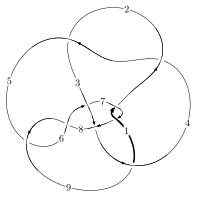
\includegraphics[width=112pt]{../../../GIT/diagram.site/Diagrams/png/73_9_38.png}\\
\ \ \ A knot diagram\footnotemark}&
\allowdisplaybreaks
\textbf{Linearized knot diagam} \\
\cline{2-2}
 &
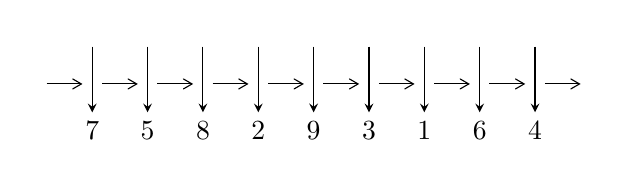
\begin{tikzpicture}[x=20pt, y=17pt]
	% nodes
	\node (C0) at (0, 0) {};
	\node (C1) at (1, 0) {};
	\node (C1U) at (1, +1) {};
	\node (C1D) at (1, -1) {7};

	\node (C2) at (2, 0) {};
	\node (C2U) at (2, +1) {};
	\node (C2D) at (2, -1) {5};

	\node (C3) at (3, 0) {};
	\node (C3U) at (3, +1) {};
	\node (C3D) at (3, -1) {8};

	\node (C4) at (4, 0) {};
	\node (C4U) at (4, +1) {};
	\node (C4D) at (4, -1) {2};

	\node (C5) at (5, 0) {};
	\node (C5U) at (5, +1) {};
	\node (C5D) at (5, -1) {9};

	\node (C6) at (6, 0) {};
	\node (C6U) at (6, +1) {};
	\node (C6D) at (6, -1) {3};

	\node (C7) at (7, 0) {};
	\node (C7U) at (7, +1) {};
	\node (C7D) at (7, -1) {1};

	\node (C8) at (8, 0) {};
	\node (C8U) at (8, +1) {};
	\node (C8D) at (8, -1) {6};

	\node (C9) at (9, 0) {};
	\node (C9U) at (9, +1) {};
	\node (C9D) at (9, -1) {4};
	\node (C10) at (10, 0) {};

	% arrows
	\draw[->,>={angle 60}]
	(C0) edge (C1) (C1) edge (C2) (C2) edge (C3) (C3) edge (C4) (C4) edge (C5) (C5) edge (C6) (C6) edge (C7) (C7) edge (C8) (C8) edge (C9) (C9) edge (C10) ;	\draw[->,>=stealth]
	(C1U) edge (C1D) (C2U) edge (C2D) (C3U) edge (C3D) (C4U) edge (C4D) (C5U) edge (C5D) (C6U) edge (C6D) (C7U) edge (C7D) (C8U) edge (C8D) (C9U) edge (C9D) ;
	\end{tikzpicture} \\
\hhline{~~} \\& 
\textbf{Solving Sequence} \\ \cline{2-2} 
 &
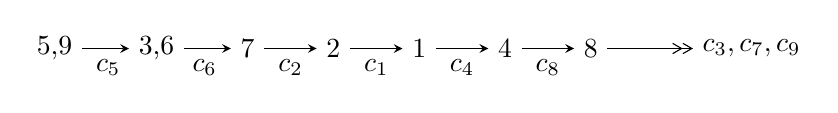
\begin{tikzpicture}[x=31pt, y=7pt]
	% node
	\node (A0) at (-1/8, 0) {5,9};
	\node (A1) at (17/16, 0) {3,6};
	\node (A2) at (17/8, 0) {7};
	\node (A3) at (25/8, 0) {2};
	\node (A4) at (33/8, 0) {1};
	\node (A5) at (41/8, 0) {4};
	\node (A6) at (49/8, 0) {8};
	\node (C1) at (1/2, -1) {$c_{5}$};
	\node (C2) at (13/8, -1) {$c_{6}$};
	\node (C3) at (21/8, -1) {$c_{2}$};
	\node (C4) at (29/8, -1) {$c_{1}$};
	\node (C5) at (37/8, -1) {$c_{4}$};
	\node (C6) at (45/8, -1) {$c_{8}$};
	\node (A7) at (8, 0) {$c_{3},c_{7},c_{9}$};

	% edge
	\draw[->,>=stealth]	
	(A0) edge (A1) (A1) edge (A2) (A2) edge (A3) (A3) edge (A4) (A4) edge (A5) (A5) edge (A6) ;
	\draw[->>,>={angle 60}]	
	(A6) edge (A7);
\end{tikzpicture} \\ 

\end{tabular} \\

\footnotetext{
The image of knot diagram is generated by the software ``\textbf{Draw programme}" developed by Andrew Bartholomew(\url{http://www.layer8.co.uk/maths/draw/index.htm\#Running-draw}), where we modified some parts for our purpose(\url{https://github.com/CATsTAILs/LinksPainter}).
}\phantom \\ \newline 
\centering \textbf{Ideals for irreducible components\footnotemark of $X_{\text{par}}$} 
 
\begin{align*}
I^u_{1}&=\langle 
- u^{10}-2 u^9-5 u^8-11 u^7-14 u^6-20 u^5-23 u^4-16 u^3-13 u^2+4 b-4 u+1,\\
\phantom{I^u_{1}}&\phantom{= \langle  }u^{10}+2 u^9+5 u^8+11 u^7+10 u^6+12 u^5+15 u^4-7 u^2+8 a-4 u-9,\\
\phantom{I^u_{1}}&\phantom{= \langle  }u^{11}+u^{10}+3 u^9+6 u^8+7 u^7+10 u^6+11 u^5+9 u^4+9 u^3+3 u^2+3 u+1\rangle \\
I^u_{2}&=\langle 
20020 u^{17}-48508 u^{16}+\cdots+11959 b-19142,\;-16736 u^{17}+49970 u^{16}+\cdots+11959 a-645,\\
\phantom{I^u_{2}}&\phantom{= \langle  }u^{18}-3 u^{17}+\cdots-2 u+1\rangle \\
I^u_{3}&=\langle 
b+1,\;2 a+1,\;u-1\rangle \\
\\
\end{align*}
\raggedright * 3 irreducible components of $\dim_{\mathbb{C}}=0$, with total 30 representations.\\
\footnotetext{All coefficients of polynomials are rational numbers. But the coefficients are sometimes approximated in decimal forms when there is not enough margin.}
\newpage
\renewcommand{\arraystretch}{1}
\centering \section*{I. $I^u_{1}= \langle - u^{10}-2 u^9+\cdots+4 b+1,\;u^{10}+2 u^9+\cdots+8 a-9,\;u^{11}+u^{10}+\cdots+3 u+1 \rangle$}
\flushleft \textbf{(i) Arc colorings}\\
\begin{tabular}{m{7pt} m{180pt} m{7pt} m{180pt} }
\flushright $a_{5}=$&$\begin{pmatrix}1\\0\end{pmatrix}$ \\
\flushright $a_{9}=$&$\begin{pmatrix}0\\u\end{pmatrix}$ \\
\flushright $a_{3}=$&$\begin{pmatrix}-\frac{1}{8} u^{10}-\frac{1}{4} u^9+\cdots+\frac{1}{2} u+\frac{9}{8}\\\frac{1}{4} u^{10}+\frac{1}{2} u^9+\cdots+u-\frac{1}{4}\end{pmatrix}$ \\
\flushright $a_{6}=$&$\begin{pmatrix}1\\u^2\end{pmatrix}$ \\
\flushright $a_{7}=$&$\begin{pmatrix}-\frac{1}{16} u^{10}-\frac{1}{8} u^9+\cdots-\frac{7}{4} u+\frac{1}{16}\\-\frac{1}{8} u^{10}-\frac{1}{4} u^9+\cdots-\frac{1}{2} u+\frac{1}{8}\end{pmatrix}$ \\
\flushright $a_{2}=$&$\begin{pmatrix}\frac{1}{8} u^{10}+\frac{1}{4} u^9+\cdots+\frac{3}{2} u+\frac{7}{8}\\\frac{1}{4} u^{10}+\frac{1}{2} u^9+\cdots+u-\frac{1}{4}\end{pmatrix}$ \\
\flushright $a_{1}=$&$\begin{pmatrix}\frac{1}{16} u^{10}+\frac{1}{8} u^9+\cdots+\frac{7}{4} u+\frac{15}{16}\\\frac{1}{8} u^{10}+\frac{1}{4} u^9+\cdots+\frac{3}{2} u-\frac{1}{8}\end{pmatrix}$ \\
\flushright $a_{4}=$&$\begin{pmatrix}\frac{3}{8} u^{10}+\frac{3}{4} u^9+\cdots+\frac{5}{2} u+\frac{13}{8}\\\frac{5}{4} u^{10}+\frac{3}{2} u^9+\cdots+u-\frac{1}{4}\end{pmatrix}$ \\
\flushright $a_{8}=$&$\begin{pmatrix}u\\u^3+u\end{pmatrix}$\\ \flushright $a_{8}=$&$\begin{pmatrix}u\\u^3+u\end{pmatrix}$\\&\end{tabular}
\flushleft \textbf{(ii) Obstruction class $= -1$}\\~\\
\flushleft \textbf{(iii) Cusp Shapes $= -\frac{27}{16} u^{10}+\frac{13}{8} u^9-\frac{23}{16} u^8-\frac{41}{16} u^7+\frac{37}{8} u^6+\frac{7}{4} u^5-\frac{13}{16} u^4+7 u^3-\frac{3}{16} u^2+\frac{31}{4} u-\frac{181}{16}$}\\~\\
\newpage\renewcommand{\arraystretch}{1}
\flushleft \textbf{(iv) u-Polynomials at the component}\newline \\
\begin{tabular}{m{50pt}|m{274pt}}
Crossings & \hspace{64pt}u-Polynomials at each crossing \\
\hline $$\begin{aligned}c_{1},c_{5},c_{7}\\c_{8}\end{aligned}$$&$\begin{aligned}
&u^{11}+u^{10}+3 u^9+6 u^8+7 u^7+10 u^6+11 u^5+9 u^4+9 u^3+3 u^2+3 u+1
\end{aligned}$\\
\hline $$\begin{aligned}c_{2},c_{4}\end{aligned}$$&$\begin{aligned}
&u^{11}-3 u^9+u^8+4 u^7-2 u^6- u^5+10 u^4-5 u^3-16 u^2+9 u+4
\end{aligned}$\\
\hline $$\begin{aligned}c_{3}\end{aligned}$$&$\begin{aligned}
&u^{11}-3 u^{10}+\cdots-6 u+8
\end{aligned}$\\
\hline $$\begin{aligned}c_{6},c_{9}\end{aligned}$$&$\begin{aligned}
&2(2 u^{11}+u^{10}-3 u^8+11 u^7+2 u^6-14 u^5+7 u^4+6 u^3-5 u^2+1)
\end{aligned}$\\
\hline
\end{tabular}\\~\\
\newpage\renewcommand{\arraystretch}{1}
\flushleft \textbf{(v) Riley Polynomials at the component}\newline \\
\begin{tabular}{m{50pt}|m{274pt}}
Crossings & \hspace{64pt}Riley Polynomials at each crossing \\
\hline $$\begin{aligned}c_{1},c_{5},c_{7}\\c_{8}\end{aligned}$$&$\begin{aligned}
&y^{11}+5 y^{10}+11 y^9+8 y^8-5 y^7+47 y^5+87 y^4+73 y^3+27 y^2+3 y-1
\end{aligned}$\\
\hline $$\begin{aligned}c_{2},c_{4}\end{aligned}$$&$\begin{aligned}
&y^{11}-6 y^{10}+\cdots+209 y-16
\end{aligned}$\\
\hline $$\begin{aligned}c_{3}\end{aligned}$$&$\begin{aligned}
&y^{11}+3 y^{10}+\cdots+52 y-64
\end{aligned}$\\
\hline $$\begin{aligned}c_{6},c_{9}\end{aligned}$$&$\begin{aligned}
&4(4 y^{11}- y^{10}+\cdots+10 y-1)
\end{aligned}$\\
\hline
\end{tabular}\\~\\
\newpage\flushleft \textbf{(vi) Complex Volumes and Cusp Shapes}
$$\begin{array}{c|c|c}  
\text{Solutions to }I^u_{1}& \I (\text{vol} + \sqrt{-1}CS) & \text{Cusp shape}\\
 \hline 
\begin{aligned}
u &= -0.361784 + 0.962924 I \\
a &= \phantom{-}0.42885 - 1.90311 I \\
b &= -1.019420 + 0.904921 I\end{aligned}
 & \phantom{-}0.53843 + 4.57539 I & -8.21994 - 7.99945 I \\ \hline\begin{aligned}
u &= -0.361784 - 0.962924 I \\
a &= \phantom{-}0.42885 + 1.90311 I \\
b &= -1.019420 - 0.904921 I\end{aligned}
 & \phantom{-}0.53843 - 4.57539 I & -8.21994 + 7.99945 I \\ \hline\begin{aligned}
u &= -1.186630 + 0.355210 I \\
a &= \phantom{-}0.360998 + 0.003803 I \\
b &= \phantom{-}0.988348 + 0.222965 I\end{aligned}
 & -3.44203 - 0.72668 I & -9.61068 + 7.91738 I \\ \hline\begin{aligned}
u &= -1.186630 - 0.355210 I \\
a &= \phantom{-}0.360998 - 0.003803 I \\
b &= \phantom{-}0.988348 - 0.222965 I\end{aligned}
 & -3.44203 + 0.72668 I & -9.61068 - 7.91738 I \\ \hline\begin{aligned}
u &= \phantom{-}0.256965 + 0.681325 I \\
a &= \phantom{-}0.565680 + 0.993565 I \\
b &= -1.41820 - 0.12736 I\end{aligned}
 & -1.48009 - 1.36667 I & -10.72983 + 4.40179 I \\ \hline\begin{aligned}
u &= \phantom{-}0.256965 - 0.681325 I \\
a &= \phantom{-}0.565680 - 0.993565 I \\
b &= -1.41820 + 0.12736 I\end{aligned}
 & -1.48009 + 1.36667 I & -10.72983 - 4.40179 I \\ \hline\begin{aligned}
u &= \phantom{-}0.391610 + 1.210140 I \\
a &= -0.57189 + 1.31384 I \\
b &= \phantom{-}0.308687 - 1.224930 I\end{aligned}
 & \phantom{-}6.41512 - 6.30680 I & -3.61485 + 5.61897 I \\ \hline\begin{aligned}
u &= \phantom{-}0.391610 - 1.210140 I \\
a &= -0.57189 - 1.31384 I \\
b &= \phantom{-}0.308687 + 1.224930 I\end{aligned}
 & \phantom{-}6.41512 + 6.30680 I & -3.61485 - 5.61897 I \\ \hline\begin{aligned}
u &= \phantom{-}0.57851 + 1.29417 I \\
a &= -0.05089 - 1.59336 I \\
b &= \phantom{-}1.29294 + 0.67490 I\end{aligned}
 & \phantom{-}3.25113 - 12.93290 I & -6.73085 + 7.81031 I \\ \hline\begin{aligned}
u &= \phantom{-}0.57851 - 1.29417 I \\
a &= -0.05089 + 1.59336 I \\
b &= \phantom{-}1.29294 - 0.67490 I\end{aligned}
 & \phantom{-}3.25113 + 12.93290 I & -6.73085 - 7.81031 I\\
 \hline 
 \end{array}$$\newpage$$\begin{array}{c|c|c}  
\text{Solutions to }I^u_{1}& \I (\text{vol} + \sqrt{-1}CS) & \text{Cusp shape}\\
 \hline 
\begin{aligned}
u &= -0.357337\phantom{ +0.000000I} \\
a &= \phantom{-}1.03450\phantom{ +0.000000I} \\
b &= -0.304704\phantom{ +0.000000I}\end{aligned}
 & -0.695510\phantom{ +0.000000I} & -14.4380\phantom{ +0.000000I}\\
 \hline 
 \end{array}$$\newpage\newpage\renewcommand{\arraystretch}{1}
\centering \section*{II. $I^u_{2}= \langle 20020 u^{17}-48508 u^{16}+\cdots+11959 b-19142,\;-16736 u^{17}+49970 u^{16}+\cdots+11959 a-645,\;u^{18}-3 u^{17}+\cdots-2 u+1 \rangle$}
\flushleft \textbf{(i) Arc colorings}\\
\begin{tabular}{m{7pt} m{180pt} m{7pt} m{180pt} }
\flushright $a_{5}=$&$\begin{pmatrix}1\\0\end{pmatrix}$ \\
\flushright $a_{9}=$&$\begin{pmatrix}0\\u\end{pmatrix}$ \\
\flushright $a_{3}=$&$\begin{pmatrix}1.39945 u^{17}-4.17844 u^{16}+\cdots+1.61753 u+0.0539343\\-1.67405 u^{17}+4.05619 u^{16}+\cdots-1.50280 u+1.60064\end{pmatrix}$ \\
\flushright $a_{6}=$&$\begin{pmatrix}1\\u^2\end{pmatrix}$ \\
\flushright $a_{7}=$&$\begin{pmatrix}-0.146501 u^{17}+0.631491 u^{16}+\cdots-2.98386 u+4.22619\\-0.318087 u^{17}+1.15194 u^{16}+\cdots-0.807425 u-0.186972\end{pmatrix}$ \\
\flushright $a_{2}=$&$\begin{pmatrix}-0.274605 u^{17}-0.122251 u^{16}+\cdots+0.114725 u+1.65457\\-1.67405 u^{17}+4.05619 u^{16}+\cdots-1.50280 u+1.60064\end{pmatrix}$ \\
\flushright $a_{1}=$&$\begin{pmatrix}-3.02350 u^{17}+9.06932 u^{16}+\cdots-5.85985 u+4.11447\\-1.51769 u^{17}+3.28171 u^{16}+\cdots+1.19801 u+0.319257\end{pmatrix}$ \\
\flushright $a_{4}=$&$\begin{pmatrix}2.04465 u^{17}-5.56234 u^{16}+\cdots+1.85467 u-1.18196\\-0.318087 u^{17}+1.15194 u^{16}+\cdots-0.807425 u-0.186972\end{pmatrix}$ \\
\flushright $a_{8}=$&$\begin{pmatrix}u\\u^3+u\end{pmatrix}$\\ \flushright $a_{8}=$&$\begin{pmatrix}u\\u^3+u\end{pmatrix}$\\&\end{tabular}
\flushleft \textbf{(ii) Obstruction class $= -1$}\\~\\
\flushleft \textbf{(iii) Cusp Shapes $= \frac{35580}{11959} u^{17}-\frac{72112}{11959} u^{16}+\cdots+\frac{57268}{11959} u-\frac{174278}{11959}$}\\~\\
\newpage\renewcommand{\arraystretch}{1}
\flushleft \textbf{(iv) u-Polynomials at the component}\newline \\
\begin{tabular}{m{50pt}|m{274pt}}
Crossings & \hspace{64pt}u-Polynomials at each crossing \\
\hline $$\begin{aligned}c_{1},c_{5},c_{7}\\c_{8}\end{aligned}$$&$\begin{aligned}
&u^{18}-3 u^{17}+\cdots-2 u+1
\end{aligned}$\\
\hline $$\begin{aligned}c_{2},c_{4}\end{aligned}$$&$\begin{aligned}
&(u^9- u^8-2 u^7+3 u^6+u^5-3 u^4+2 u^3- u+1)^2
\end{aligned}$\\
\hline $$\begin{aligned}c_{3}\end{aligned}$$&$\begin{aligned}
&(u^9+u^8+2 u^7+u^6+3 u^5+u^4+2 u^3+u-1)^2
\end{aligned}$\\
\hline $$\begin{aligned}c_{6},c_{9}\end{aligned}$$&$\begin{aligned}
&u^{18}-3 u^{17}+\cdots+4 u+11
\end{aligned}$\\
\hline
\end{tabular}\\~\\
\newpage\renewcommand{\arraystretch}{1}
\flushleft \textbf{(v) Riley Polynomials at the component}\newline \\
\begin{tabular}{m{50pt}|m{274pt}}
Crossings & \hspace{64pt}Riley Polynomials at each crossing \\
\hline $$\begin{aligned}c_{1},c_{5},c_{7}\\c_{8}\end{aligned}$$&$\begin{aligned}
&y^{18}+11 y^{17}+\cdots+14 y^2+1
\end{aligned}$\\
\hline $$\begin{aligned}c_{2},c_{4}\end{aligned}$$&$\begin{aligned}
&(y^9-5 y^8+12 y^7-15 y^6+9 y^5+y^4-4 y^3+2 y^2+y-1)^2
\end{aligned}$\\
\hline $$\begin{aligned}c_{3}\end{aligned}$$&$\begin{aligned}
&(y^9+3 y^8+8 y^7+13 y^6+17 y^5+17 y^4+12 y^3+6 y^2+y-1)^2
\end{aligned}$\\
\hline $$\begin{aligned}c_{6},c_{9}\end{aligned}$$&$\begin{aligned}
&y^{18}+7 y^{17}+\cdots+1260 y+121
\end{aligned}$\\
\hline
\end{tabular}\\~\\
\newpage\flushleft \textbf{(vi) Complex Volumes and Cusp Shapes}
$$\begin{array}{c|c|c}  
\text{Solutions to }I^u_{2}& \I (\text{vol} + \sqrt{-1}CS) & \text{Cusp shape}\\
 \hline 
\begin{aligned}
u &= -0.131255 + 1.025520 I \\
a &= \phantom{-}2.21228 - 3.01855 I \\
b &= -0.825933\phantom{ +0.000000I}\end{aligned}
 & \phantom{-}2.09142\phantom{ +0.000000I} & -12.65235 + 0. I\phantom{ +0.000000I} \\ \hline\begin{aligned}
u &= -0.131255 - 1.025520 I \\
a &= \phantom{-}2.21228 + 3.01855 I \\
b &= -0.825933\phantom{ +0.000000I}\end{aligned}
 & \phantom{-}2.09142\phantom{ +0.000000I} & -12.65235 + 0. I\phantom{ +0.000000I} \\ \hline\begin{aligned}
u &= \phantom{-}1.068960 + 0.157811 I \\
a &= \phantom{-}0.330746 + 0.183937 I \\
b &= \phantom{-}1.172470 - 0.500383 I\end{aligned}
 & -0.30826 + 7.08493 I & -9.57680 - 5.91335 I \\ \hline\begin{aligned}
u &= \phantom{-}1.068960 - 0.157811 I \\
a &= \phantom{-}0.330746 - 0.183937 I \\
b &= \phantom{-}1.172470 + 0.500383 I\end{aligned}
 & -0.30826 - 7.08493 I & -9.57680 + 5.91335 I \\ \hline\begin{aligned}
u &= \phantom{-}0.255037 + 0.861194 I \\
a &= \phantom{-}0.31995 + 1.69908 I \\
b &= -1.173910 - 0.391555 I\end{aligned}
 & -1.08148 - 1.33617 I & -11.28409 + 0.70175 I \\ \hline\begin{aligned}
u &= \phantom{-}0.255037 - 0.861194 I \\
a &= \phantom{-}0.31995 - 1.69908 I \\
b &= -1.173910 + 0.391555 I\end{aligned}
 & -1.08148 + 1.33617 I & -11.28409 - 0.70175 I \\ \hline\begin{aligned}
u &= -0.287150 + 1.197360 I \\
a &= -0.077942 - 1.012210 I \\
b &= \phantom{-}0.141484 + 0.739668 I\end{aligned}
 & \phantom{-}2.67293 + 2.45442 I & -6.32792 - 2.91298 I \\ \hline\begin{aligned}
u &= -0.287150 - 1.197360 I \\
a &= -0.077942 + 1.012210 I \\
b &= \phantom{-}0.141484 - 0.739668 I\end{aligned}
 & \phantom{-}2.67293 - 2.45442 I & -6.32792 + 2.91298 I \\ \hline\begin{aligned}
u &= \phantom{-}0.605058 + 1.127080 I \\
a &= \phantom{-}0.639032 - 1.048120 I \\
b &= \phantom{-}0.772920 + 0.510351 I\end{aligned}
 & \phantom{-}5.07330 - 2.09337 I & -3.48501 + 4.16283 I \\ \hline\begin{aligned}
u &= \phantom{-}0.605058 - 1.127080 I \\
a &= \phantom{-}0.639032 + 1.048120 I \\
b &= \phantom{-}0.772920 - 0.510351 I\end{aligned}
 & \phantom{-}5.07330 + 2.09337 I & -3.48501 - 4.16283 I\\
 \hline 
 \end{array}$$\newpage$$\begin{array}{c|c|c}  
\text{Solutions to }I^u_{2}& \I (\text{vol} + \sqrt{-1}CS) & \text{Cusp shape}\\
 \hline 
\begin{aligned}
u &= \phantom{-}0.658024 + 0.097431 I \\
a &= \phantom{-}0.910679 + 0.215358 I \\
b &= \phantom{-}0.141484 - 0.739668 I\end{aligned}
 & \phantom{-}2.67293 - 2.45442 I & -6.32792 + 2.91298 I \\ \hline\begin{aligned}
u &= \phantom{-}0.658024 - 0.097431 I \\
a &= \phantom{-}0.910679 - 0.215358 I \\
b &= \phantom{-}0.141484 + 0.739668 I\end{aligned}
 & \phantom{-}2.67293 + 2.45442 I & -6.32792 - 2.91298 I \\ \hline\begin{aligned}
u &= -0.62758 + 1.28014 I \\
a &= \phantom{-}0.023182 + 1.259910 I \\
b &= \phantom{-}1.172470 - 0.500383 I\end{aligned}
 & -0.30826 + 7.08493 I & -9.57680 - 5.91335 I \\ \hline\begin{aligned}
u &= -0.62758 - 1.28014 I \\
a &= \phantom{-}0.023182 - 1.259910 I \\
b &= \phantom{-}1.172470 + 0.500383 I\end{aligned}
 & -0.30826 - 7.08493 I & -9.57680 + 5.91335 I \\ \hline\begin{aligned}
u &= \phantom{-}0.31006 + 1.39846 I \\
a &= -0.515395 + 0.355009 I \\
b &= \phantom{-}0.772920 - 0.510351 I\end{aligned}
 & \phantom{-}5.07330 + 2.09337 I & -3.48501 - 4.16283 I \\ \hline\begin{aligned}
u &= \phantom{-}0.31006 - 1.39846 I \\
a &= -0.515395 - 0.355009 I \\
b &= \phantom{-}0.772920 + 0.510351 I\end{aligned}
 & \phantom{-}5.07330 - 2.09337 I & -3.48501 + 4.16283 I \\ \hline\begin{aligned}
u &= -0.351155 + 0.305986 I \\
a &= \phantom{-}1.157480 - 0.200845 I \\
b &= -1.173910 - 0.391555 I\end{aligned}
 & -1.08148 - 1.33617 I & -11.28409 + 0.70175 I \\ \hline\begin{aligned}
u &= -0.351155 - 0.305986 I \\
a &= \phantom{-}1.157480 + 0.200845 I \\
b &= -1.173910 + 0.391555 I\end{aligned}
 & -1.08148 + 1.33617 I & -11.28409 - 0.70175 I\\
 \hline 
 \end{array}$$\newpage\newpage\renewcommand{\arraystretch}{1}
\centering \section*{III. $I^u_{3}= \langle b+1,\;2 a+1,\;u-1 \rangle$}
\flushleft \textbf{(i) Arc colorings}\\
\begin{tabular}{m{7pt} m{180pt} m{7pt} m{180pt} }
\flushright $a_{5}=$&$\begin{pmatrix}1\\0\end{pmatrix}$ \\
\flushright $a_{9}=$&$\begin{pmatrix}0\\1\end{pmatrix}$ \\
\flushright $a_{3}=$&$\begin{pmatrix}-0.5\\-1\end{pmatrix}$ \\
\flushright $a_{6}=$&$\begin{pmatrix}1\\1\end{pmatrix}$ \\
\flushright $a_{7}=$&$\begin{pmatrix}1.25\\1.5\end{pmatrix}$ \\
\flushright $a_{2}=$&$\begin{pmatrix}-1.5\\-1\end{pmatrix}$ \\
\flushright $a_{1}=$&$\begin{pmatrix}-0.25\\0.5\end{pmatrix}$ \\
\flushright $a_{4}=$&$\begin{pmatrix}-0.5\\-1\end{pmatrix}$ \\
\flushright $a_{8}=$&$\begin{pmatrix}1\\2\end{pmatrix}$\\ \flushright $a_{8}=$&$\begin{pmatrix}1\\2\end{pmatrix}$\\&\end{tabular}
\flushleft \textbf{(ii) Obstruction class $= 1$}\\~\\
\flushleft \textbf{(iii) Cusp Shapes $= -9.75$}\\~\\
\newpage\renewcommand{\arraystretch}{1}
\flushleft \textbf{(iv) u-Polynomials at the component}\newline \\
\begin{tabular}{m{50pt}|m{274pt}}
Crossings & \hspace{64pt}u-Polynomials at each crossing \\
\hline $$\begin{aligned}c_{1},c_{4},c_{8}\end{aligned}$$&$\begin{aligned}
&u+1
\end{aligned}$\\
\hline $$\begin{aligned}c_{2},c_{5},c_{7}\end{aligned}$$&$\begin{aligned}
&u-1
\end{aligned}$\\
\hline $$\begin{aligned}c_{3}\end{aligned}$$&$\begin{aligned}
&u
\end{aligned}$\\
\hline $$\begin{aligned}c_{6}\end{aligned}$$&$\begin{aligned}
&2(2 u+1)
\end{aligned}$\\
\hline $$\begin{aligned}c_{9}\end{aligned}$$&$\begin{aligned}
&2(2 u-1)
\end{aligned}$\\
\hline
\end{tabular}\\~\\
\newpage\renewcommand{\arraystretch}{1}
\flushleft \textbf{(v) Riley Polynomials at the component}\newline \\
\begin{tabular}{m{50pt}|m{274pt}}
Crossings & \hspace{64pt}Riley Polynomials at each crossing \\
\hline $$\begin{aligned}c_{1},c_{2},c_{4}\\c_{5},c_{7},c_{8}\end{aligned}$$&$\begin{aligned}
&y-1
\end{aligned}$\\
\hline $$\begin{aligned}c_{3}\end{aligned}$$&$\begin{aligned}
&y
\end{aligned}$\\
\hline $$\begin{aligned}c_{6},c_{9}\end{aligned}$$&$\begin{aligned}
&4(4 y-1)
\end{aligned}$\\
\hline
\end{tabular}\\~\\
\newpage\flushleft \textbf{(vi) Complex Volumes and Cusp Shapes}
$$\begin{array}{c|c|c}  
\text{Solutions to }I^u_{3}& \I (\text{vol} + \sqrt{-1}CS) & \text{Cusp shape}\\
 \hline 
\begin{aligned}
u &= \phantom{-}1.00000\phantom{ +0.000000I} \\
a &= -0.500000\phantom{ +0.000000I} \\
b &= -1.00000\phantom{ +0.000000I}\end{aligned}
 & -3.28987\phantom{ +0.000000I} & -9.75000\phantom{ +0.000000I}\\
 \hline 
 \end{array}$$\newpage
\newpage\renewcommand{\arraystretch}{1}
\centering \section*{ IV. u-Polynomials}
\begin{tabular}{m{50pt}|m{274pt}}
Crossings & \hspace{64pt}u-Polynomials at each crossing \\
\hline $$\begin{aligned}c_{1},c_{8}\end{aligned}$$&$\begin{aligned}
&(u+1)\\
&\cdot(u^{11}+u^{10}+3 u^9+6 u^8+7 u^7+10 u^6+11 u^5+9 u^4+9 u^3+3 u^2+3 u+1)\\
&\cdot(u^{18}-3 u^{17}+\cdots-2 u+1)
\end{aligned}$\\
\hline $$\begin{aligned}c_{2}\end{aligned}$$&$\begin{aligned}
&(u-1)(u^9- u^8-2 u^7+3 u^6+u^5-3 u^4+2 u^3- u+1)^2\\
&\cdot(u^{11}-3 u^9+u^8+4 u^7-2 u^6- u^5+10 u^4-5 u^3-16 u^2+9 u+4)
\end{aligned}$\\
\hline $$\begin{aligned}c_{3}\end{aligned}$$&$\begin{aligned}
&u(u^9+u^8+2 u^7+u^6+3 u^5+u^4+2 u^3+u-1)^2\\
&\cdot(u^{11}-3 u^{10}+\cdots-6 u+8)
\end{aligned}$\\
\hline $$\begin{aligned}c_{4}\end{aligned}$$&$\begin{aligned}
&(u+1)(u^9- u^8-2 u^7+3 u^6+u^5-3 u^4+2 u^3- u+1)^2\\
&\cdot(u^{11}-3 u^9+u^8+4 u^7-2 u^6- u^5+10 u^4-5 u^3-16 u^2+9 u+4)
\end{aligned}$\\
\hline $$\begin{aligned}c_{5},c_{7}\end{aligned}$$&$\begin{aligned}
&(u-1)\\
&\cdot(u^{11}+u^{10}+3 u^9+6 u^8+7 u^7+10 u^6+11 u^5+9 u^4+9 u^3+3 u^2+3 u+1)\\
&\cdot(u^{18}-3 u^{17}+\cdots-2 u+1)
\end{aligned}$\\
\hline $$\begin{aligned}c_{6}\end{aligned}$$&$\begin{aligned}
&4(2 u+1)(2 u^{11}+u^{10}+\cdots-5 u^2+1)\\
&\cdot(u^{18}-3 u^{17}+\cdots+4 u+11)
\end{aligned}$\\
\hline $$\begin{aligned}c_{9}\end{aligned}$$&$\begin{aligned}
&4(2 u-1)(2 u^{11}+u^{10}+\cdots-5 u^2+1)\\
&\cdot(u^{18}-3 u^{17}+\cdots+4 u+11)
\end{aligned}$\\
\hline
\end{tabular}\newpage\renewcommand{\arraystretch}{1}
\centering \section*{ V. Riley Polynomials}
\begin{tabular}{m{50pt}|m{274pt}}
Crossings & \hspace{64pt}Riley Polynomials at each crossing \\
\hline $$\begin{aligned}c_{1},c_{5},c_{7}\\c_{8}\end{aligned}$$&$\begin{aligned}
&(y-1)\\
&\cdot(y^{11}+5 y^{10}+11 y^9+8 y^8-5 y^7+47 y^5+87 y^4+73 y^3+27 y^2+3 y-1)\\
&\cdot(y^{18}+11 y^{17}+\cdots+14 y^2+1)
\end{aligned}$\\
\hline $$\begin{aligned}c_{2},c_{4}\end{aligned}$$&$\begin{aligned}
&(y-1)(y^9-5 y^8+12 y^7-15 y^6+9 y^5+y^4-4 y^3+2 y^2+y-1)^2\\
&\cdot(y^{11}-6 y^{10}+\cdots+209 y-16)
\end{aligned}$\\
\hline $$\begin{aligned}c_{3}\end{aligned}$$&$\begin{aligned}
&y(y^9+3 y^8+8 y^7+13 y^6+17 y^5+17 y^4+12 y^3+6 y^2+y-1)^2\\
&\cdot(y^{11}+3 y^{10}+\cdots+52 y-64)
\end{aligned}$\\
\hline $$\begin{aligned}c_{6},c_{9}\end{aligned}$$&$\begin{aligned}
&16(4 y-1)(4 y^{11}-y^{10}+\cdots+10 y-1)(y^{18}+7 y^{17}+\cdots+1260 y+121)
\end{aligned}$\\
\hline
\end{tabular}
\vskip 2pc
\end{document}